%Het eerste hoofdstuk van je thesis.
\chapter{Opdrachtbeschrijving}
De opdracht bestaat erin om een line-following robot te maken. De opdracht was iets anders dan de klassieke line-follower, we konden namelijk geen volle lijn volgen. De baan bestond uit twee volle lijnen met er tussenin een stippellijn, de breedte van de baan is ongeveer twee keer de breedte van de auto. We kregen al de carrosserie van de auto, samen met de twee motoren en een batterij. We mochten zoveel componenten 3D printen zoals we wouden. We kregen een budget van 50 euro ter beschikking. We kunnen de opdracht opsplitsen in twee takken, hardware en software.
\section{Hardware}
We moesten natuurlijk zelf zorgen voor de elektronica. We konden om de opdracht uit te werken gebruik maken van een Arduino Uno gecombineerd met een Motorshield van Sparksfun, zie figuur~\ref{fig:ArduMoto}. Maar uiteindelijk moesten we zelf selecteren uit de Arduino en de Motorshield wat we nodig hadden en er zelf 1 printplaat te maken. Voor de sensors, de Bluetooth-module en de RFID-reader mochten we kiezen of we zelf dingen ontworpen of kant-en-klare modules te kopen.
\begin{figure}[h]
\centering
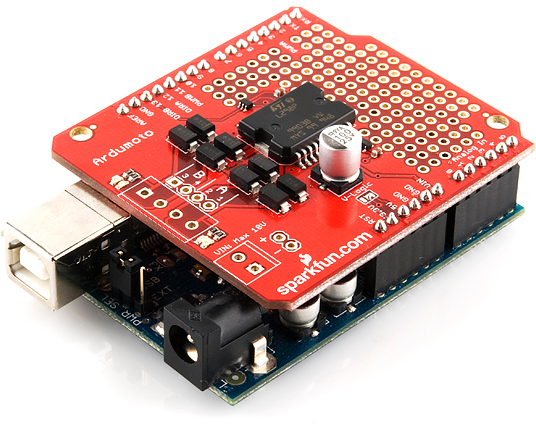
\includegraphics[width=0.75\textwidth]{ArduMoto.png}
\caption{Motorshield gecombineerd met een Arduino. \label{fig:ArduMoto}}
\end{figure}
\section{Software}
Het tweede onderdeel van de onderdeel bestond erin om de arduino (en dus later ook onze eigen PCB) te programmeren. We moesten gebruik maken van PID-afregeling. We moesten ook de snelheid kunnen meten, RFID-tags uitlezen en dit alles doorsturen via Bluetooth naar een Raspberry Pi.
%In dit hoofdstuk\index{hoofdstuk} gaan we een voorbeeld geven van een voetnoot\footnote{Dit is dus een voetnoot}. Een referentie naar hoofdstuk ~\ref{verwijzing}, dat zich op pagina \pageref{verwijzing} bevindt, is dus ook een koud kunstje. Zorg er wel voor dat je de namen van de labels een beetje verstandig kiest. Hoofdstukken label je het best als hfdstk:naam, plaatjes als img:naam en tabellen\index{tabellen} als tabel:naam. Zo verlies je zelf de bomen in het bos niet.
%\newpage
%SDffjfhd fsffh hsf
%fh fhf
%shf klfh
%ffffsdfklfhklfhklfhhfklfhkldhffhsdfhfhfhfhfh
%\newpage
%dhfhffh hf fh fh fhfh fhfh hfh fhffhsdfhfhfhfhfhfhsdfh hfh fh
 



